\documentclass[11pt, oneside]{article}   	% use "amsart" instead of "article" for AMSLaTeX format
\usepackage[margin = 1in]{geometry}                		% See geometry.pdf to learn the layout options. There are lots.
\geometry{letterpaper}                   		% ... or a4paper or a5paper or ... 
%\geometry{landscape}                		% Activate for rotated page geometry
\usepackage[parfill]{parskip}    		% Activate to begin paragraphs with an empty line rather than an indent
\usepackage{graphicx, ulem, tikz, multicol}				% Use pdf, png, jpg, or eps§ with pdflatex; use eps in DVI mode
								% TeX will automatically convert eps --> pdf in pdflatex		
\usepackage{amssymb, enumerate}

%SetFonts

%SetFonts


\title{Math F113X: Homework Set 7}
%\author{The Author}
\date{}							% Activate to display a given date or no date

\begin{document}
\maketitle
%\section{}
%\subsection{}

%Homework assignment 1 is:
%\vspace{-1.5cm}


\fbox{\parbox{\textwidth}{

\begin{itemize}
\item \textbf{Section:} Graph Theory  \\
\textbf{Topic: } Algorithms for finding Hamiltonian circuits \\
\# 19*, 22*, A, B, C \\

* In part b of both of these problems, you should complete Nearest Neighbor on \textbf{TWO} additional vertices. After that, you can use the solutions to determine which vertex gives a minimum for this algorithm.\\

\item \textbf{Section:} Scheduling \\
\textbf{Topic:} Introduction to Scheduling \\
\#1, 2, 3, 6
\end{itemize}
}}

\quad\\

\textbf{Problem A:} Answer questions about the graph below.

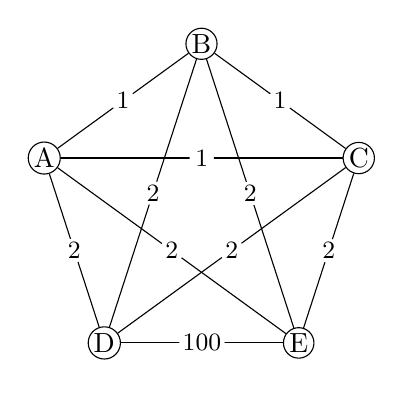
\begin{tikzpicture}[scale=.7,
  every node/.style={circle, draw, fill=white, minimum size=1mm,inner sep=.5pt},
  every edge/.style={draw},
  edge label/.style={draw=none, fill=white, font=\small, inner sep=.5pt}
]

% Place 5 vertices in a pentagon
\node (B) at (90:3)  {B};
\node (C) at (18:3)  {C};
\node (E) at (306:3) {E};
\node (D) at (234:3) {D};
\node (A) at (162:3) {A};

% Weight-1 edges: between A, B, C (i.e. AB, AC, BC)
\draw (A) -- node[edge label] {1} (B);
\draw (A) -- node[edge label] {1} (C);
\draw (B) -- node[edge label] {1} (C);

% Weight-100 edge: D--E
\draw (D) -- node[edge label] {100} (E);

% Weight-2 edges: all remaining pairs
% Pairs involving D or E with A, B, C, and cross pairs not already listed
\draw (A) -- node[edge label] {2} (D);
\draw (A) -- node[edge label] {2} (E);
\draw (B) -- node[edge label] {2} (D);
\draw (B) -- node[edge label] {2} (E);
\draw (C) -- node[edge label] {2} (D);
\draw (C) -- node[edge label] {2} (E);

\end{tikzpicture}
	\begin{enumerate}
	\item Apply the Repeated Nearest Neighbor Algorithm and determine the weight of the resulting circuit. (Note that you are allowed to use symmetry in the graph to make this faster!)
	\item Apply the Sorted Edges Algorithm and determine the weight of the resulting circuit.
	\item Using your own judgment, find a minimum weight Hamiltonian circuit.
	\item Does either algorithm --  Repeated Nearest Neighbor or Sorted Edges -- return a minimum weight Hamiltonian circuit?
	\end{enumerate} 
	
\textbf{Problem B:} Create weighted, complete 5-vertex graph with vertex set $A$, $B$, $C$, $D$, and $E,$ such that the Nearest Neighbor algorithm starting at $A$ will give an optimal solution but starting at $B$ will give the worst possible solution. Show your answer is correct. \\

\textbf{Problem C:} Suppose someone wants to visit the capital city of every state in the contiguous 48 states and Washington DC. So, they will visit 49 cities in total. [NOTE: you will need to use a computational tool, like WolframAlpha, to complete this problem.]
	\begin{enumerate}
	\item Suppose they want to start and end the 49-city-tour at the same place. How many different tours are possible? (Your answer should be in \emph{both} factorial notation and in scientific notation.)
	\item Suppose you have a computer that can calculate the length of 1000 49-city-tours in one second. How long would it take the computer to calculate the length of all possible 49-city-tours? Give your answer in \emph{years}. 
	\item What does your answer in part $2$ indicate about the Brute Force algorithm?
	\end{enumerate}


\hrulefill

Remember to write up your homework solutions according to the homework writeup guidelines. 

Homework is graded using the following rubric for each problem (or problem part):

\begin{description}
\item[2 points:] You provided a complete answer, with supporting work, written up clearly
\item[1 point:] Some attempt at a solution, but incomplete writeup / unclear / illegible / no answer
\item[1 point:] Only an answer, with no supporting work 
\item[0 points:] Missing.
\end{description}

After you do the homework, you need to check your answers against the solutions! Then figure out your errors (if any) and revise your homework before you submit it. 

Homework must be submitted on Gradescope.

\end{document}  